\PassOptionsToPackage{xetex}{xcolor}
\PassOptionsToPackage{xetex}{graphicx}
\documentclass[a4paper,landscape,headrule,footrule,xetex,25pt]{foils}

%%
%%%  Macros
%%%
\newcommand{\logo}{~}
\MyLogo{HG8011 (2019)}
\newcommand{\Story}{\SHA{HOUN}{The Hound of the Baskervilles}}

\newcommand{\header}[3]{%
\title{\vspace*{-2ex} \large Detecting Meaning with Sherlock Holmes\thanks{Creative Commons Attribution License: you are free to share and adapt as long as you give appropriate credit and add no additional restrictions: 
\protect\url{https://creativecommons.org/licenses/by/4.0/}.}
%\footnotemark
\\[2ex] \Large  \emp{#2} \\ \emp{#3}}
\author{\blu{Francis Bond}   \\ 
\normalsize  \textbf{Division of Linguistics and Multilingual Studies}\\
\normalsize  \url{http://www3.ntu.edu.sg/home/fcbond/}\\
\normalsize  \texttt{bond@ieee.org}}
 \date{Location: LT25}
 \renewcommand{\logo}{#2}
 \hypersetup{
   pdfinfo={
     Author={Francis Bond},
     Title={#2},
     Subject={HG8011: Detecting Meaning with Sherlock Holmes},
     Keywords={Semantics, Pragmatics, Meaning},
     License={CC BY 4.0}
   }
 %  pdfcopyright={Copyright © Francis Bond. Creative Commons 4.0 Attribution License.}
 %  pdflicenseurl={http://creativecommons.org/licenses/by/4.0/}
 }
}
%%
%% Multilingual Stuff
%%
\usepackage[a4paper,landscape,margin=25mm]{geometry}

\usepackage{fontenc}
\usepackage{polyglossia}
\setmainlanguage{english}
\setmainfont{TeX Gyre Pagella}
\usepackage{xeCJK}
\setCJKmainfont{Noto Sans CJK SC}
\setCJKsansfont{Noto Sans CJK SC}
\setCJKmonofont{Noto Sans CJK SC}
%\setCJKttfont{Noto Sans CJK SC}
%\setCJKmainfont{WenQuanYi Micro Hei}
%\clearpage
%\setCJKmainfont{AR PL SungtiL GB}

\usepackage[xetex]{xcolor}
\usepackage[xetex]{graphicx}
\newcommand{\blu}[1]{\textcolor{blue}{#1}}
\newcommand{\grn}[1]{\textcolor{green}{#1}}
\newcommand{\hide}[1]{\textcolor{white}{#1}}
\newcommand{\emp}[1]{\textcolor{red}{#1}}
\newcommand{\txx}[1]{\textbf{\textcolor{blue}{#1}}}
\newcommand{\lex}[1]{\textbf{\mtcitestyle{#1}}}

\usepackage{pifont}
\renewcommand{\labelitemi}{\textcolor{violet}{\ding{227}}}
\renewcommand{\labelitemii}{\textcolor{purple}{\ding{226}}}

\newcommand{\subhead}[1]{\noindent\textbf{#1}\\[5mm]}

\newcommand{\Bad}{\emp{\raisebox{0.15ex}{\ensuremath{\mathbf{\otimes}}}}}
\newcommand{\bad}{*}

\newcommand{\com}[1]{\hfill \textnormal{(\emp{#1})}}%
\newcommand{\cxm}[1]{\hfill \textnormal{(\txx{#1})}}%
\newcommand{\cmm}[1]{\hfill \textnormal{(#1)}}%
\usepackage{amssymb}
\usepackage{relsize,xspace}
\newcommand{\into}{\ensuremath{\rightarrow}\xspace}
\newcommand{\ent}{\ensuremath{\Rightarrow}\xspace}
\newcommand{\nent}{\ensuremath{\not\Rightarrow}\xspace}
\newcommand{\tot}{\ensuremath{\leftrightarrow}\xspace}
\usepackage{url}
\usepackage[hidelinks]{hyperref}
\hypersetup{
     colorlinks,
     linkcolor={blue!50!black},
     citecolor={red!50!black},
     urlcolor={blue!80!black}
}
%\usepackage{hyperxmp}
\newcommand{\lurl}[1]{\MyLogo{\url{#1}}}

\usepackage{mygb4e}
\let\eachwordone=\itshape
\newcommand{\lx}[1]{\textbf{\textit{#1}}}
\newcommand{\ix}{\ex\it}

\newcommand{\cen}[2]{\multicolumn{#1}{c}{#2}}
%\usepackage{times}
%\usepackage{nttfoilhead}
\newcommand{\myslide}[1]{%
\foilhead[-25mm]{\raisebox{12mm}[0mm]{\emp{#1}}}%
\leftheader{}%
\MyLogo{\logo}}

\newcommand{\mytask}[1]{%
\foilhead[-25mm]{\raisebox{12mm}[0mm]{\emp{#1}}}
\leftheader{🔍 Hi}%
\MyLogo{\logo}}

\newcommand{\myslider}[1]{\rotatefoilhead[-25mm]{\raisebox{12mm}[0mm]{\emp{#1}}}}
%\newcommand{\myslider}[1]{\rotatefoilhead{\raisebox{-8mm}{\emp{#1}}}}

\newcommand{\section}[1]{\myslide{}{\begin{center}\Huge \emp{#1}\end{center}}}

\usepackage{tcolorbox}
% \newcommand{\task}{\marginpar{\raisebox{-1ex}{\large
%       \tcbox[colframe=red,colback=white,arc=3pt]{\textbf{?}}}}}
% \newcommand{\task}{\marginpar{\raisebox{-1ex}{
%       \hspace{-0.5em}\tcbox[colframe=red,colback=white,arc=3pt]{%
%         
\includegraphics[width=1.5em]{pics/detective}}}}}
\newcommand{\task}{\marginpar{\raisebox{-2ex}{
      \hspace{-0.5em}\reflectbox{
\includegraphics[width=2em]{pics/detective}}}}}

\usepackage[lyons,j,e,k]{mtg2e}
\renewcommand{\mtcitestyle}[1]{\textcolor{teal}{\textsl{#1}}}
%\renewcommand{\mtcitestyle}[1]{\textsl{#1}}
\newcommand{\chn}{\mtciteform}
\newcommand{\cmn}{\mtciteform}
\newcommand{\iz}[1]{\textup{\texttt{\textcolor{blue}{\textbf{#1}}}}}
\newcommand{\con}[1]{\textsc{#1}}
\newcommand{\gm}{\textsc}
\newcommand{\cmp}[1]{{[\textsc{#1}]}}
\newcommand{\sr}[1]{\ensuremath{\langle}#1\ensuremath{\rangle}}
\usepackage[normalem]{ulem}
\newcommand{\ul}{\uline}
\newcommand{\ull}{\uuline}
\newcommand{\wl}{\uwave}
\newcommand{\vs}{\ensuremath{\Leftrightarrow}~}
%%%
%%% Bibliography
%%%
\usepackage{natbib}
%\usepackage{url}
\usepackage{bibentry}


%%% From Tim
\newcommand{\WMngram}[1][]{$n$-gram#1\xspace}
\newcommand{\infers}{$\rightarrow$\xspace}



\usepackage{rtrees,qtree}
\renewcommand{\lf}[1]{\br{#1}{}}
\usepackage{avm}
%\avmoptions{topleft,center}
\newcommand{\ft}[1]{\textsc{#1}}
%\newcommand{\val}[1]{\textit{#1}}
\newcommand{\typ}[1]{\textit{#1}}
\avmfont{\sc}
%\avmvalfont{\sc}
\renewcommand{\avmtreefont}{\sc}
\avmsortfont{\it}


%%% From CSLI book
\newcommand{\mc}{\multicolumn}
\newcommand{\HD}{\textbf{H}\xspace}
\newcommand{\el}{\< \>}
\makeatother
\long\def\smalltree#1{\leavevmode{\def\\{\cr\noalign{\vskip12pt}}%
\def\mc##1##2{\multispan{##1}{\hfil##2\hfil}}%
\tabskip=1em%
\hbox{\vtop{\halign{&\hfil##\hfil\cr
#1\crcr}}}}}
\makeatletter

\newcommand{\sh}[1]{\lowercase{\href{https://fcbond.github.io/sh-canon/#1.html}}{#1}}
\newcommand{\SHA}[2]{\lowercase{\href{https://fcbond.github.io/sh-canon/#1.html}}{\textit{#2}}}


\begin{document}
\header{Lecture 1}{Introduction, Organization}{What does it mean to mean?}
\maketitle

%\include{schedule}


\myslide{Welcome!}

\begin{itemize}
\item In this course we will introduce you to the study of meaning
  \begin{itemize}
  \item How meaning is built up from words and phrases
  \item How meaning depends on context
  \item How to critically read texts
  \item How to appreciate the historical and cultural context of a text
  \item How stories are transformed in different media
%Understanding how cinematic elements affect our understanding
  \item  How meaning changes as it is transmitted in different languages and cultures 
  \end{itemize}
\item Using the Sherlock Homes stories (and films, \ldots{}) as examples
  \begin{itemize}
  \item Try to make this as enjoyable as possible
  \item Read (and watch) some great stories
  \end{itemize}
\end{itemize}


\myslide{The original team}
\newcommand{\picwidth}{0.16\textwidth}
\begin{center}
  \begin{tabular}{cccc}
    
\includegraphics[width=\picwidth]{pics/francis} & 
    
\includegraphics[width=\picwidth]{pics/jane} \\
    Francis Bond &
    Jane Wong, Yeang Chui \\
    % (黄仰翠)
    Semantics \& Pragmatics & Literary Analysis \\
    
\includegraphics[width=\picwidth]{pics/brian} & 
    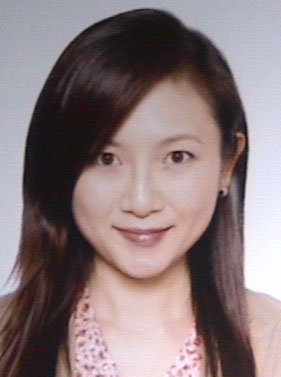
\includegraphics[width=\picwidth]{pics/uganda} \\
    Brian Keith Bergen-Aurand &
    Uganda Sze Pui Kwan & \\
    Film Theory & Translation Studies\\
    % (關詩珮).
  \end{tabular}
\end{center}


\myslide{Francis Bond}

\begin{itemize}\addtolength{\itemsep}{-1ex}
%\item Francis Bond 
\item BA in Japanese and Mathematics 
\item BEng in Power and Control %(Electrical Systems Engineering)
  \raisebox{-2ex}[0mm][0mm]{
\includegraphics{pics/pwm}}
\item PhD in English on  \textit{Determiners and Number in English
  contrasted with Japanese,  as exemplified in Machine
  Translation} 
\item 1991-2006 \textbf{NTT} (Nippon Telegraph and Telephone)
  \begin{itemize}
  \item Japanese - English/Malay Machine Translation
%  \item Japanese corpus, grammar and ontology (Hinoki)
  \end{itemize}
\item 2006-2009 \textbf{NICT} (National Inst. for Info. and Comm. Technology)
  \begin{itemize}
  \item Japanese - English/Chinese Machine Translation
%  \item Japanese WordNet
  \end{itemize}
\item 2009- \textbf{NTU} (Nanyang Technological University)
  \begin{itemize}
  \item Cross-lingual representation of meaning
  \end{itemize}

\newpage
\item Proud SOB (\href{www.soundofthebaskervilles.com/}{Sound of the
    Baskervilles})
\item Hound of the Internet
\item  \href{http://johnhwatsonsociety.com/treasure-hunt/results/}{High Honours} in the 2017 John H Watson Canonical Treasure Hunt 
  (Francis Bond, Margie Deck, Sheila Holtgrieve,
  Lauren Messenger)\footnote{Alphabetical order}

\end{itemize}



\myslide{Overview of today}

\begin{itemize}
\item How this course is organized
\item Why Sherlock Holmes
\item What is semantics
\item Why should we be interested in semantics
\item Syllabus; Administrivia
\end{itemize}

% \myslide{Course Content}

% This course introduces basic corpus skills for linguists:
% \begin{itemize}
% \item Marking up extra information
% \item Selecting text
% \item The range of existing corpora
% \item How to build your own corpus
% \item Using corpora to test linguistic hypotheses
% \item Using corpora to train language tools
% \end{itemize}




\myslide{What do you learn?}


Students will learn semantics at an introductory level and they will
acquire semantic analysis skills. With these skills and their
knowledge of semantic approaches, students will be able to approach
natural language data, as well as develop awareness of the inherent
connections between semantics and other branches of linguistics.  In
the second half of the course, we will show how the stories (and other
works adapted from them) convey meaning to the reader, as well as how
the meaning becomes part of our cultural heritage.  


\myslide{Course Content}

This course introduces basic skills in semantic and literary analysis, such as:
\begin{itemize}
\item   Distinguishing word senses
\item   Understanding how meaning is built up compositionally
\item   Understanding how words can convey feelings
\item   Understanding how meaning can be conveyed indirectly
\newpage
\item   Identify characteristics of modern detective fiction
\item   Understanding how to approach a text in a critical manner
\item   Understanding how to appreciate the historical and cultural context of a text
\item   Understanding how stories are transformed in different media
\item   Understanding how cinematic elements affect our understanding
\item   Understanding how meaning changes as it is transmitted in different languages and cultures 
\end{itemize}




\myslide{Textbook and Readings}

\begin{itemize}
\item No required text book and not much reading
\item\emp{EXCEPT you must read the stories assigned: \\ at least four,
    maybe more}
\item If you want to know more about semantics I recommend
  \begin{itemize}
  \item Saeed, John (2009). \textit{Semantics}. 3rd Edition. Wiley-Blackwell. 
  \item Lyons, John (1977) \textit{Semantics}.  Cambridge University Press
  \end{itemize}
\item Between now and next week, I expect you to read the assigned three stories.
\end{itemize}

\myslide{Studying meaning}

\begin{itemize}
\item I will teach you about meaning
\item You will then try to analyze the use of words 
  \\ in the Sherlock Holmes stories
  \begin{itemize}
  \item Word Meaning (sense)
    \\   https://lr.soh.ntu.edu.sg/ntumc/cgi-bin/showcorpus.cgi
    \\  \eng{to knock up}
  \item Word and Sentence Meaning (sentiment)
    \\  \eng{Julia and I had no great pleasure in our lives}
  \item Idioms and metaphors
    \\ \eng{to cross someone's path}
  \end{itemize}
\item You must do the three online projects, each is 4--8 hours work

\end{itemize}



% Other References

% Biber, D., S. Conrad \& R. Reppen, Corpus Linguistics: Investigating Language Structure and Use. Cambridge University Press, 1998.

% Kennedy, G. An Introduction to Corpus Linguistics. Longman, 1998.

% McEnery, Tony et al. Corpus-Based Language Studies: An Advanced Resource Book. Routledge, 2006.

% McEnery, Tony and Andrew Wilson Corpus Linguistics 2nd ed, Edinburgh UP, 2001

% Sinclair, John. Corpus Concordance Collocation. Oxford: Oxford UP, 1991



\section{Sherlock Holmes}
\begin{center}
  
\includegraphics[width=0.3\textwidth]{pics/detectiveprofile}
\end{center}

\myslide{Why Sherlock Holmes?}
\MyLogo{I want to make studying semantics more accessible}
\begin{itemize}
\item Enjoyable, reasonably straight-forward stories
\item Close enough to modern English to be readable
\item Popular enough to be easily available
\item Old enough to be out of copyright
\item Widely translated and adapted
\item Very early examples of fan-fiction and geekery
\end{itemize}

\myslide{Who is Sherlock Holmes?}
\MyLogo{\lex{ratiocination} ``logical and methodical reasoning''}
\begin{itemize}
\item A London-based consulting detective
  \raisebox{-20ex}[0ex][0ex]{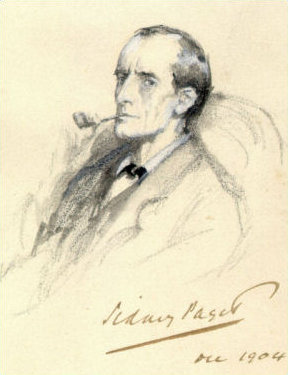
\includegraphics[width=0.3\textwidth]{pics/Sherlock_Holmes_Portrait_Paget}}
\item who solves many cases
\item with a quirky personality
\item skilled with disguises
\item with immense powers of observation and raticionation
\item and a faithful friend: John Watson
% \end{itemize}
% \begin{center}
%  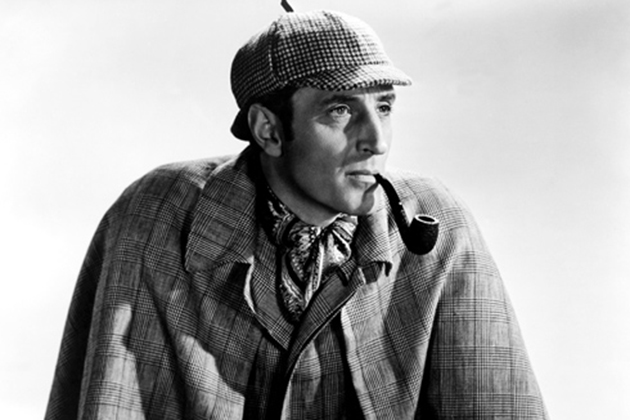
\includegraphics[width=0.3\textwidth]{pics/sherlock-holmes-basil-rathbone}
  \raisebox{-10ex}[0ex][0ex]{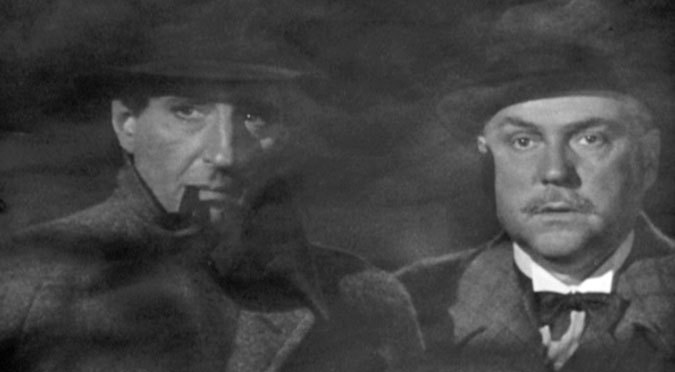
\includegraphics[width=0.4\textwidth]{pics/sherlock-holmes-john-watson}}
\item lives on 221B Baker street
%
%\end{center}
\end{itemize}

\myslide{Who is Sherlock Holmes in the real world?}
%\MyLogo{\lex{raticionation} ``logical and methodical reasoning''}

\begin{itemize}\addtolength{\itemsep}{-1ex}
\item A fictional detective, invented by Sir Arthur Conan Doyle
\item He appeared in a total of 60 stories,  published between 1887 and 1927
\item The four novels and five volumes of short stories now often
  appear as The Complete Sherlock Holmes and are referred to as \txx{the CANON}
\item Most of the stories are narrated by Holmes's friend and
  biographer, Dr. John H. Watson
\item The stories were popular then, and have remained popular
\item They have been adapted as plays, radio shows, films, tv series, manga and many, many more
\end{itemize}

\myslide{What is Sherlock like?}
\MyLogo{You will read this}
\begin{itemize}
\item Watch: Sherlock deduces the nature of a man
\item from \textit{The Red-Headed League} Season 2 Episode 5
\\  Granada Television: 1984--1994
\item First aired at 9:00 PM in the United Kingdom on Tuesday, 22 September 1985 on ITV
\item Jeremy Brett as Sherlock Holmes; David Burke as Dr. Watson; Roger Hammond as Jabez Wilson
  \begin{quote}
     “Beyond the obvious facts that he has at some time done manual labour, that he takes snuff, that he is a Freemason, that he has been in China, and that he has done a considerable amount of writing lately, I can deduce nothing else.”
  \end{quote}
\end{itemize}



% The portly client puffed out his chest with an appearance of some little pride, and pulled a dirty and wrinkled newspaper from the inside pocket of his greatcoat. As he glanced down the advertisement column, with his head thrust forward, and the paper flattened out upon his knee, I took a good look at the man, and endeavoured, after the fashion of my companion, to read the indications which might be presented by his dress or appearance.

% I did not gain very much, however, by my inspection. Our visitor bore every mark of being an average commonplace British tradesman, obese, pompous, and slow. He wore rather baggy gray shepherd's check trousers, a not overclean black frockcoat, unbuttoned in the front, and a drab waistcoat with a heavy brassy Albert chain, and a square pierced bit of metal dangling down as an ornament. A frayed top hat and a faded brown overcoat with a wrinkled velvet collar lay upon a chair beside him. Altogether, look as I would, there was nothing remarkable about the man save his blazing red head, and the expression of extreme chagrin and discontent upon his features.

% Sherlock Holmes' quick eye took in my occupation, and he shook his head with a smile as he noticed my questioning glances. “Beyond the obvious facts that he has at some time done manual labour, that he takes snuff, that he is a Freemason, that he has been in China, and that he has done a considerable amount of writing lately, I can deduce nothing else.”

% Mr. Jabez Wilson started up in his chair, with his forefinger upon the paper, but his eyes upon my companion.

% “How, in the name of good fortune, did you know all that, Mr. Holmes?” he asked. “How did you know, for example, that I did manual labour. It's as true as gospel, for I began as a ship's carpenter.”

% “Your hands, my dear sir. Your right hand is quite a size larger than your left. You have worked with it, and the muscles are more developed.”

% “Well, the snuff, then, and the Freemasonry?”

% “I won't insult your intelligence by telling you how I read that, especially as, rather against the strict rules of your order, you use an arc and compass breastpin.”

% “Ah, of course, I forgot that. But the writing?”

% “What else can be indicated by that right cuff so very shiny for five inches, and the left one with the smooth patch near the elbow where you rest it upon the desk.”

% “Well, but China?”

% “The fish which you have tattooed immediately above your right wrist could only have been done in China. I have made a small study of tattoo marks, and have even contributed to the literature of the subject. That trick of staining the fishes' scales of a delicate pink is quite peculiar to China. When, in addition, I see a Chinese coin hanging from your watch-chain, the matter becomes even more simple.”

% Mr. Jabez Wilson laughed heavily. “Well, I never!” said he. “I thought at first that you had done something clever, but I see that there was nothing in it after all.”


\myslide{Sir Arthur Conan Doyle}

\begin{itemize}
\item \txx{Deputy Lieutenant Sir Arthur Ignatius Conan Doyle}
  \\  (22 May, 1859 – 7 July, 1930)
\item a Scottish physician and writer
\item he also wrote science fiction stories, historical novels, plays and romances, poetry, and non-fiction
\item he stood for parliament and was a crusader for reform (both in
  the army and in criminal justice)
\item he was an ardent spiritualist, and believed you could communicate with the dead.
\end{itemize}

\myslide{Doyle's relation to Sherlock Holmes}

\begin{itemize}
\item He preferred his historical fiction to Sherlock holmes
\item In fact he got so sick of the character he killed him in a short story (\textit{The Final Problem}, 1893)
\item But he needed the money, so started to write about him again from 1900 (with \textit{The Hound of the Baskervilles})
\item The last stories were published in 1926
\end{itemize}


\myslide{The inspiration for the character}

\begin{itemize}
\item  Doyle's university teacher, Dr Joseph Bell
\item Bell was born in 1837 into a family of surgeons, and at eighteen accepted a place at the Edinburgh Medical School.
\item There he was taught to observe patients very closely; and it was this attention to detail that he practised throughout his life.
  \begin{quotation}
    
Bell once remarked to an astonished outpatient: “I know you are a beadle and ring the bells on Sundays at a church in Northumberland somewhere near the Tweed.” “I'm all that,” said the man, “but how do you know? I never told you.” The outpatient left, bewildered.

Bell turned to his students: “Did you notice the Northumbrian burr in his speech, too soft for the south of Northumberland? One only finds it near the Tweed. And then his hands. Did you not notice the callosities on them caused by the ropes? Also, this is Saturday, and when I asked him if he could not come back on Monday, he said he must be getting home tonight. Then I knew he had to ring the bells tomorrow. Quite easy, gentleman, if you will only observe and put two and two together.” 
\end{quotation}
\item Doyle sent a copy of each Sherlock Holmes story to Bell in Edinburgh.
% Bell was intrigued by all the publicity and praise, but he gave all the credit to Doyle who he praised as “a born story-teller” whose genius had enabled him to make “a great deal out of very little.” 
\end{itemize}

Hume, Robert (4 November 2011). "Fiction imitates real life in a case of true inspiration". Irish Examiner. 
\url{http://www.irishexaminer.com/analysis/}
\url{fiction-imitates-real-life-in-a-case-of}
\url{-true-inspiration-172752.html} 
Retrieved 19 January 2014.

\myslide{The impact of the character}
\MyLogo{From the \href{https://www.arthur-conan-doyle.com/index.php/Sherlock_Holmes_-_The_Complete_Long_Stories}{preface for \textit{Sherlock Holmes - The
      Complete Long Stories}} Conan Doyle (1929)}

The Study in Scarlet was the first completed long story which I ever
wrote, though I had served an apprenticeship of nearly ten years of
short stories, most of which were anonymous. It represented a reaction
against the too facile way in which the detective of the old school,
so far as he was depicted in literature, gained his results. Having
endured a severe course of training in medical diagnosis, I felt that
if the same austere methods of observation and reasoning were applied
to the problems of crime some more scientific system could be
constructed.
\newpage
On the whole, taking the series of books, my view has
been justified, as I understand that in several countries some change
has been made in police procedure on account of these stories. It is
all very well to sneer at the paper detective, but a principle is a
principle, whether in fiction or in fact. Many of the great lessons of
life are to be learned in the pages of the novelist.



\section{Introduction to Semantics}

\myslide{What is Semantics}
\begin{itemize}
\item Very broadly, semantics is the study of meaning
  \begin{itemize}
  \item Word meaning
  \item Sentence meaning
  \end{itemize}
\item Why do we want to study meaning?
\item What kind of knowledge does it take for a speaker to produce language and for a hearer to comprehend language? 
\end{itemize}

\myslide{Layers of Linguistic Analysis}
\begin{enumerate}\addtolength{\itemsep}{-0.75ex}
\item Phonetics \& Phonology
\item Morphology
\item Syntax
\item Semantics
\item Pragmatics
\item Stylistics
\end{enumerate}
% Two theories
% \begin{itemize}
% \item Semantics is \txx{autonomous}, a separate module
% \item Semantics is \txx{integrated} with other knowledge, inseparable
%   \begin{itemize}
%   \item linguistic knowledge is inseparable from encyclopedic knowledge
%   \end{itemize}
% \end{itemize}

\myslide{Do people share a common conceptual system?}

\begin{itemize}
\item What is a \lex{high school}?
\item What color is \lex{blue}?
\item What does \lex{verb} mean?
\item What is  \lex{carrot cake}?
\end{itemize}

\newpage

Japanese traffic lights are green (as required by international
agreements).  However they are typically called 青い \jpn[blue]{aoi},
the same word as the color of the sky.  Historically this color
historically covered both green and blue ``grue'',
with 緑 \jpn[green]{midori} being a later addition.  For this reason,
the Japanese government decided in 1973 to change the color of the go
light to the bluest possible hue of green!


\href{https://www.japantimes.co.jp/life/2013/02/25/language/the-japanese-traffic-light-blues-stop-on-red-go-on-what/#.WRmAuuWGNPZ}{The Japanese traffic light blues: Stop on red, go on what?}
 

%\includegraphics[width=\textwidth]{pics/verbing.eps}

\myslide{Meaning is an open-ended conceptual system}

\begin{itemize}
\item Lexical innovation
  \begin{itemize}
  \item \lex{Meritocracy} (1958)
  \item \lex{LASER} (1960)
  \item \lex{WWW}
  \item[\ldots]
  \end{itemize}
\item   Is this association between creating new words and creating new concepts justified?
\item More creativity
  \begin{itemize}
  \item \eng{I am so hungry I can eat ten million elephants.}
  \end{itemize}
\end{itemize}

\myslide{\textbf{Meaning} is}
\MyLogo{Leech (1981)}

\begin{itemize}
\item An intrinsic property of a word
\item The other words annexed to a word in the dictionary
\item The connotation of a word
\item The place of anything in a system
\item The practical consequences of a thing in our future experiences
\newpage
\item That to which the user of a symbol
  \begin{itemize}
  \item actually refers to
  \item ought to be referring
  \item believes themself to be referring
  \end{itemize}
\item That to which the interpreter of a symbol
  \begin{itemize}
  \item (a) refers
  \item (b) believes themself to be referring
  \item (c) believes the user to be referring
  \end{itemize}
\end{itemize}

\myslide{More Meaning}
\begin{quotation}
  We can define the meaning of a speech form accurately when this
  meaning has to do with some matter of which we possess scientific
  knowledge. We can define the names of minerals, for example, in
  terms of chemistry and mineralogy, as when we say that the ordinary
  meaning of the English word \eng{salt} is `sodium chloride (NaCl)', and we
  can define the names of plants or animals by means of the technical
  terms of botany or zoology, but we have no precise way of defining
  words like \eng{love} or \eng{hate}, which concern situations that have not been
  accurately classified – and these latter are in the great majority.
				
\hfill				(Bloomfield, in \textit{Language} 1933)
\end{quotation}

\begin{itemize}
\item But is \lex{salt} really just NaCl?
\end{itemize}

\myslide{Determining meaning}

Some useful concepts

\begin{itemize}
\item \txx{Synonymy}: $A$ means the same as $B$
\item \txx{Contradiction}:  $A$ and $B$ cannot both be true
\item \txx{Entailment}: if  $A$ is true then  $B$ must also be true
\item \txx{Ambiguous}: $A$ has more than one meaning
\end{itemize}

\myslide{Meaning in the larger context}
\MyLogo{Most language is arbitrary.}
\begin{itemize}
\item Semiotics is the study of interpreting symbols, or \txx{signification}
  \begin{itemize}
  \item We refer to the \txx{signified}
  \item Using a \txx{signifier}\hfill Saussure
  \end{itemize}
\item Signs can be more or less related to their objects
\\  \begin{tabular}[lcc]{lllc}
    \txx{icon} & map or diagram & Children Crossing &
    
\includegraphics[width=0.1\textwidth]{pics/ryanlerch-children-crossing-road-sign.pdf} 
\\
 \txx{index} &closely represented & Roundabout &
    
\includegraphics[width=0.1\textwidth]{pics/ryanlerch-Roundabout-Sign.pdf} 
\\
   \txx{symbol} &arbitrary& Stop &
    
\includegraphics[width=0.1\textwidth]{pics/StopSign-nofont.pdf} 
    
\includegraphics[width=0.1\textwidth]{pics/Japanese-stop-sign.pdf} 
  \end{tabular}
\end{itemize}

\myslide{Problems with defining meaning}

\begin{itemize}
\item The \txx{grounding} problem and \txx{circularity}
\item The boundaries of meaning: \txx{linguistic} vs \txx{encyclopedic knowledge}
\item Regional variation in meaning: \txx{dialects} ``the usage or vocabulary that is characteristic of a specific group of people''
\item Individual variation in meaning: 
\txx{idiolects} ``the language or speech of one individual at a particular period in life''
\end{itemize}

\myslide{Metalanguages and Notational Conventions}

We use language to talk about language, which can get messy.  So we
try to use certain words with very specific technical senses.

\begin{itemize}
\item \txx{technical term} $\leftarrow$ remember me!
\item \eng[gloss]{word} or \eng{utterance}
\item \lex{lexeme}
\item \iz{predicate}
\end{itemize}

\myslide{Word Meaning and Sentence Meaning}

\begin{itemize}
\item We store information about words in our \txx{mental lexicon}
  \begin{itemize}
  \item It is still unclear what exactly a word is!
  \end{itemize}
\item Words can be combined to form an infinite number of expressions
  \begin{itemize}
  \item This building up of meaning is referred to as \txx{composition}
  \item If the meaning of the whole can be deduced from the parts then it is \txx{compositional}
  \end{itemize}
\end{itemize}

\myslide{Reference and Sense}

\begin{itemize}
\item Words \txx{refer} to things in the world (like \iz{unicorn}s)
\item The meaning of a word across different contexts is often referred to as its \txx{sense}
  \begin{itemize}
  \item Same word can refer to different things
    \begin{itemize}
    \item English: \eng{I put my money in the \ul{bank}}
    \item English: \eng{I fell asleep at the river \ul{bank}}
    \end{itemize}
  \item Same basic concept can have different boundaries
    \begin{itemize}
    \item French: \eng[sheep/mutton]{mouton}
    \item English: \eng{sheep} vs \eng{mutton}
      
    \item Japanese: \eng[dove/pigeon]{hato}
    \item English: \eng{dove} vs \eng{pigeon}
    \end{itemize}
  \end{itemize}
\end{itemize}

\myslide{Utterances, Sentences and Propositions}

\begin{itemize}
\item \txx{utterance}: an actual instance of saying (or writing  or \ldots) something
\item \txx{sentence}: an abstraction, the type of what was said
  \begin{exe}
    \ex Caesar invades Gaul
  \end{exe}
\item \txx{proposition}: a further abstraction, normally ignoring some non-literal meaning
  \begin{exe}
    \ex \iz{invade(Caesar, Gaul)}
  \end{exe}
\newpage
\item \txx{information structure}: what part of a proposition is emphasized
  \begin{exe}
   \ex \eng{Caesar invaded Gaul}
   \ex \eng{Gaul was invaded by Caesar}
   \ex \eng{It was Gaul that  Caesar invaded}
   \ex \eng{It was Caesar who invaded Gaul}
  \end{exe}
\end{itemize}


\myslide{Propositions}
\begin{itemize}
\item A logical construct
\item Abstracts away from grammatical differences
\begin{exe}
  \ex \eng{John kicked the dog}
  \ex \eng{The dog was kicked by John}
  \ex  \jpn{ジョンが犬を蹴った.} \jpn{John-ga inu-wo ketta.}
\end{exe}
\item Can be reasoned over (\txx{logic})
\item Can be formalized
\\ \iz{∃x,y(named(John,x),dog(y),the(y),kick(e,x,y),past(e))}
\end{itemize}

% \myslide{Non-literal meaning}
% \begin{itemize}
% \item Consider “That Mitchell  and Webb Look”
% \\ Season One Episode Two 1:10--
% \begin{itemize}
% \item Why aren't they more direct?
% \item Is the meaning clear anyway?
% \end{itemize}
% \item Can you give some examples of non-literal meaning?
% \end{itemize}

\myslide{Video: The Blackberry Sketch}
\MyLogo{The One Ronnie}

\begin{itemize}
\item Define the following:
  \begin{itemize}
  \item \lex{blackberry}
  \item \lex{orange}
  \item \lex{apple}
  \item \lex{date}
  \end{itemize}
\item How similar are your definitions to the use in the video?
\end{itemize}




\myslide{Representing meaning}
\MyLogo{Also vector space, description, images, video, \ldots}
\begin{itemize}
\item One of our goals will be to represent meaning
\item There are various ways to do this
  \begin{itemize}
  \item Syntactic trees
  \item Logical forms
  \item Thesauri and Ontologies 
  \item Translation
  \item Paraphrasing
  \end{itemize}
Can you think of others?

\item At the end of this course you should be able to use these to
  describe many aspects of meaning
\end{itemize}



\myslide{Language is normally under-specified}
\MyLogo{There are many meanings}
\begin{center}
\large We get \blu{words}: \\[2ex]
    \Large \eng{I saw a kid with a cat.} \\[3ex]
We want \emp{meaning}:
\\  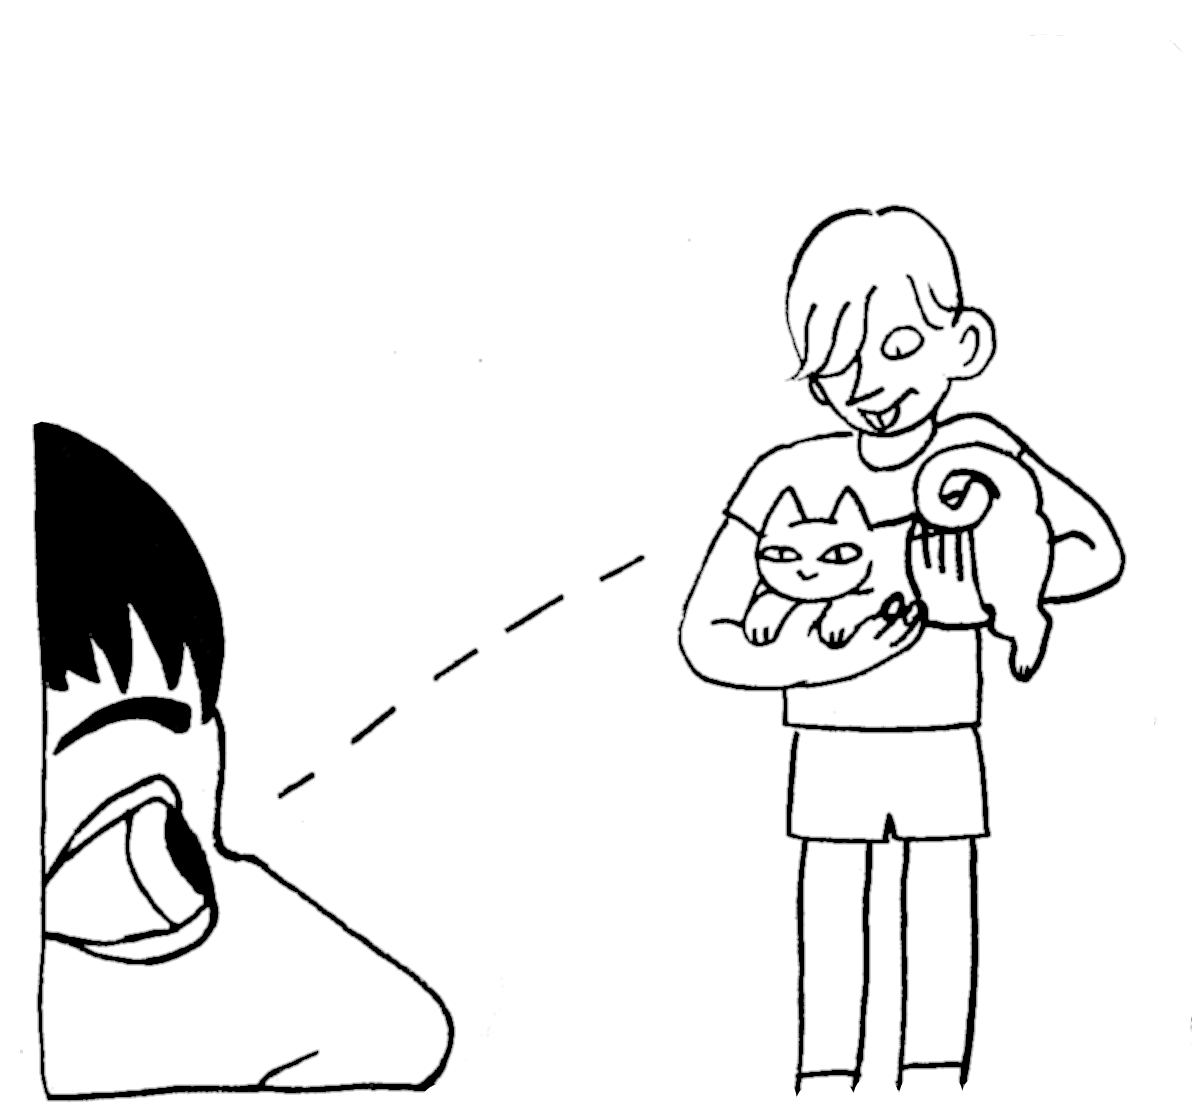
\includegraphics[width=0.3\textwidth]{pics/1.png}
\end{center}



\myslide{I saw a kid with a cat$_1$}
\MyLogo{Thanks to Eddy and Zina Pozen for the pictures}
\hspace{-3em}\begin{tabular}{ll}

  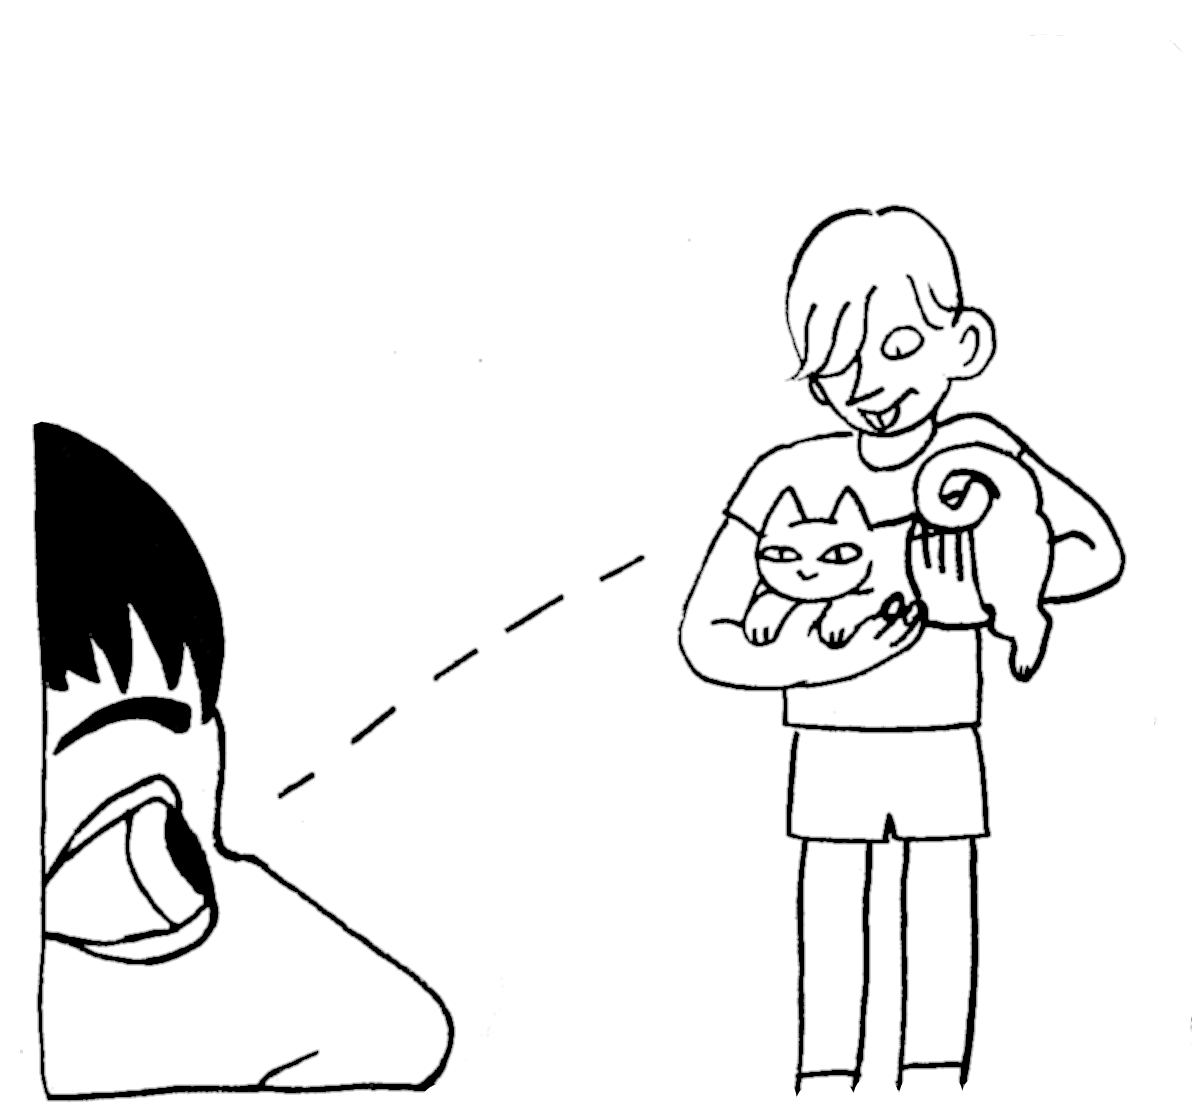
\includegraphics[width=0.5\textwidth]{pics/1.png}
&
  \begin{minipage}{0.45\textwidth}
    \vspace*{-30ex}
\begin{scriptsize}
 {%
 \leaf{\emph{I}}
 \branch{1}{NP}
 \leaf{\emph{saw}}
 \branch{1}{V:see}
 \leaf{\emph{a}}
 \branch{1}{DET}
 \leaf{\emph{kid}}
 \branch{1}{N}
 \leaf{\emph{with a cat}}
\branch{1}{PP[together]}
\branch{2}{\ibar{N}}
\branch{2}{NP}
 \branch{2}{VP}
 \branch{2}{S}
 \qobitree}
\end{scriptsize}
\\[5ex]
 \small \iz{see(I, kid: \textsc{past});  with(kid, cat)}
\\[1ex] \iz{see $\subset$ perceive}
\\ \iz{kid $\sim$ child}
\\ \iz{with $\subset$ together}
\end{minipage}

\end{tabular}

\myslide{I saw a kid with a cat$_2$}
\MyLogo{}
\hspace{-3em}\begin{tabular}{ll}
  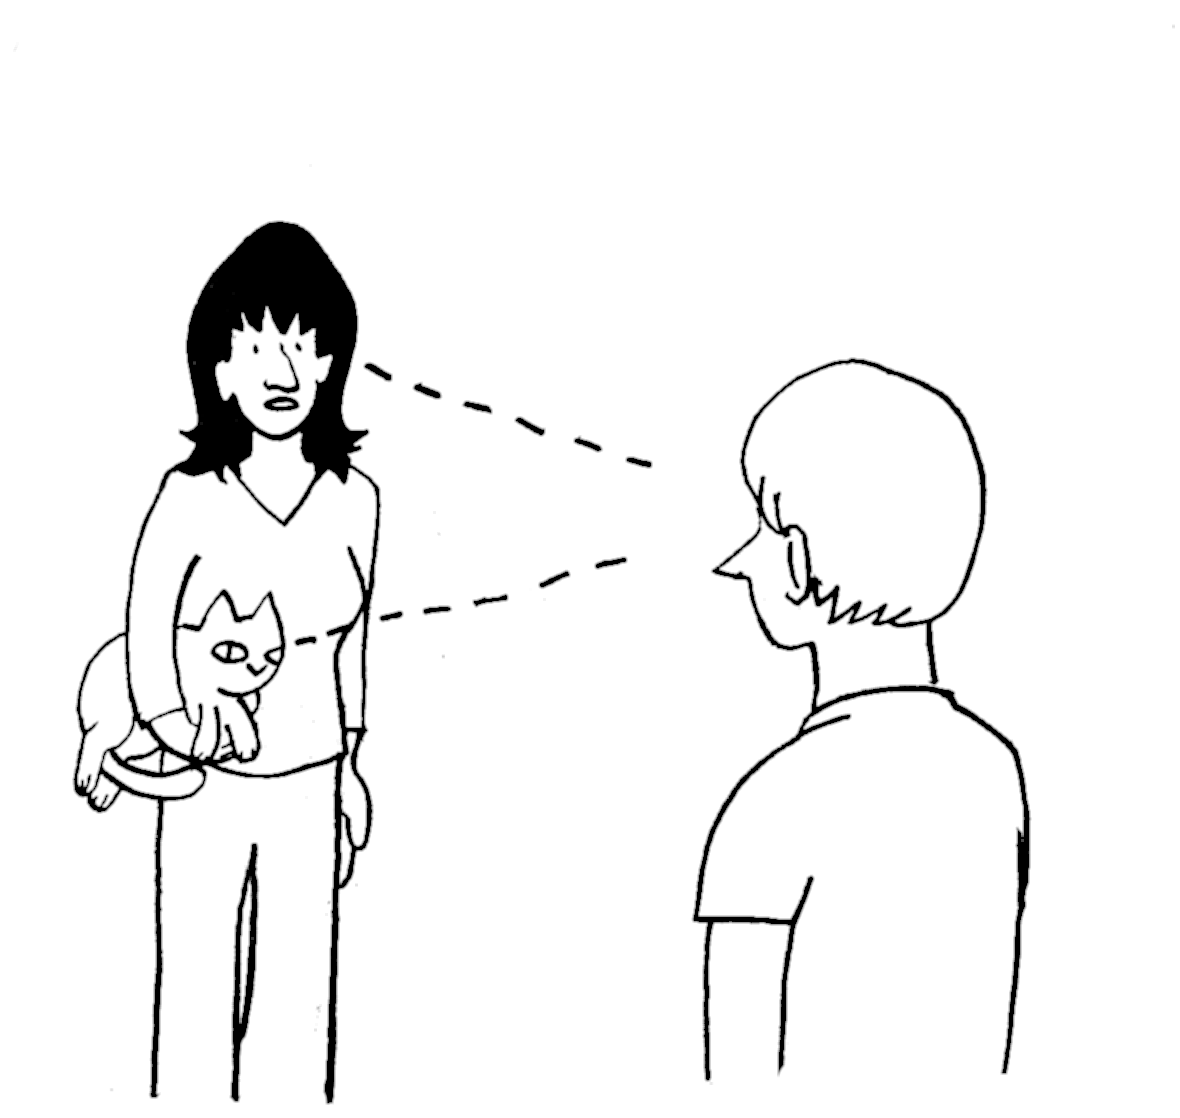
\includegraphics[width=0.5\textwidth]{pics/2.png}
&
  \begin{minipage}{0.45\textwidth}
    \vspace*{-35ex}
\begin{scriptsize}
 {%
 \leaf{\emph{I}}
 \branch{1}{NP}
 \leaf{\emph{saw}}
 \branch{1}{V:see}
 \leaf{\emph{a}}
 \branch{1}{DET}
 \leaf{\emph{kid}}
 \branch{1}{N}
\branch{2}{NP}
 \leaf{\emph{with a cat}}
\branch{1}{PP[together]}
 \branch{3}{VP}
 \branch{2}{S}
 \qobitree}
\end{scriptsize}
\\[3ex]
 \small 
 \iz{see(I, kid: \textsc{past}) with(I, cat)}
\\[1ex] \iz{see $\subset$ perceive}
\\ \iz{kid $\sim$ child}
\\ \iz{with $\subset$ together}
\end{minipage}
\end{tabular}




\myslide{I saw a kid with a cat$_3$}
\hspace{-3em}\begin{tabular}{ll}
  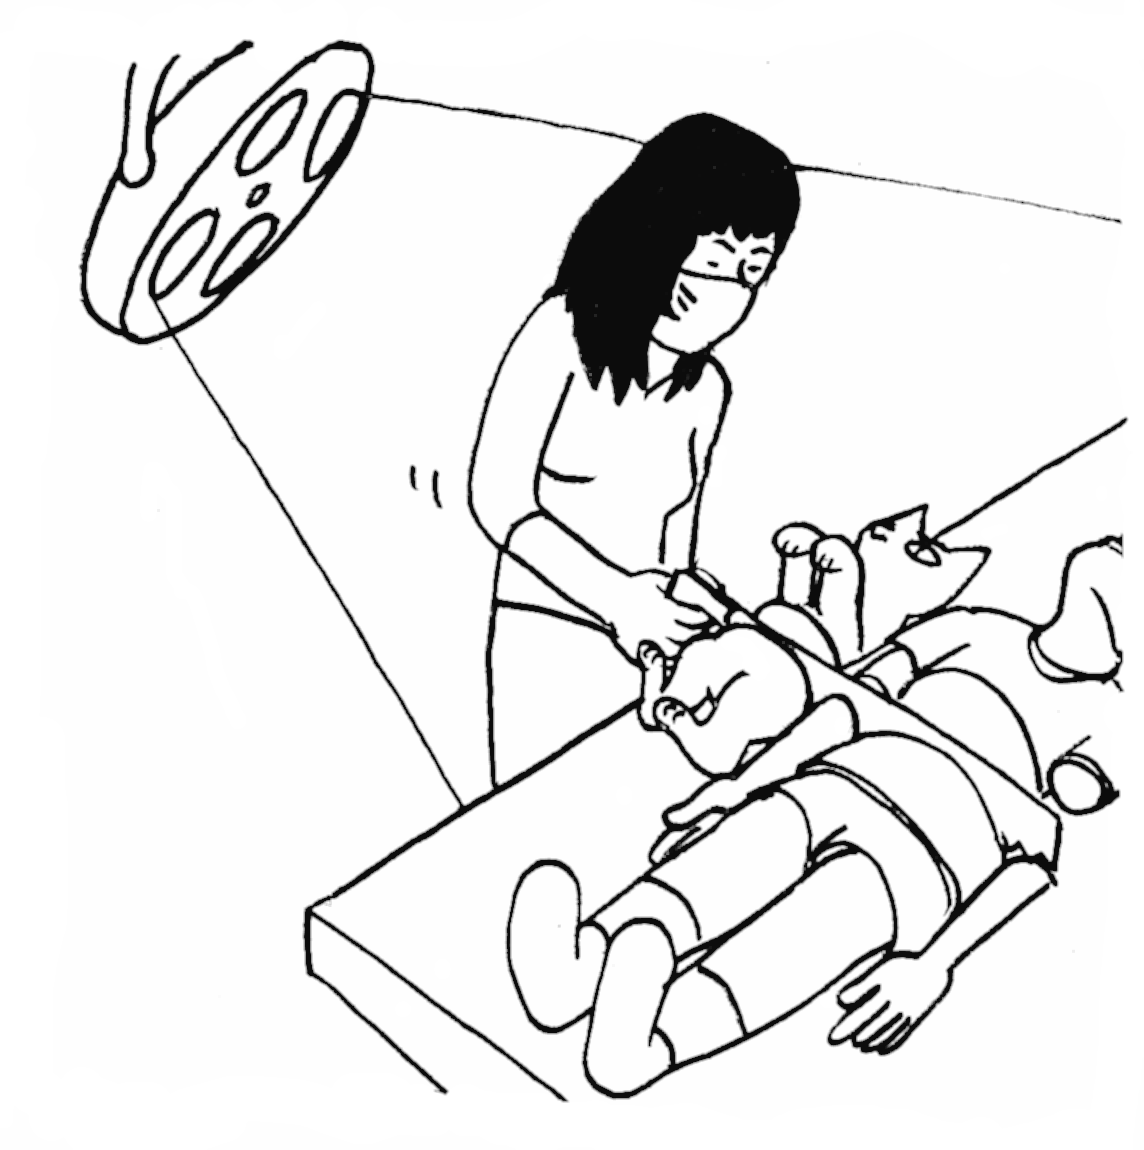
\includegraphics[width=0.5\textwidth]{pics/3.png}

&
  \begin{minipage}{0.45\textwidth}
    \vspace*{-35ex}
\begin{scriptsize}
 {%
 \leaf{\emph{I}}
 \branch{1}{NP}
 \leaf{\emph{saw}}
 \branch{1}{V:saw}
 \leaf{\emph{a}}
 \branch{1}{DET}
 \leaf{\emph{kid}}
 \branch{1}{N}
 \leaf{\emph{with a cat}}
\branch{1}{PP[together]}
\branch{2}{\ibar{N}}
\branch{2}{NP}
 \branch{2}{VP}
 \branch{2}{S}
 \qobitree}
\end{scriptsize}
\\[5ex]
 \small 
\iz{saw(I, kid: \textsc{pres});  with(kid, cat)}
\\[1ex] \iz{saw $\subset$ cut}
\\ \iz{kid $\sim$ child}
\\ \iz{with $\subset$ together}
\end{minipage}
\end{tabular}



\myslide{I saw a kid with a cat$_4$}
\hspace{-3em}\begin{tabular}{ll}
  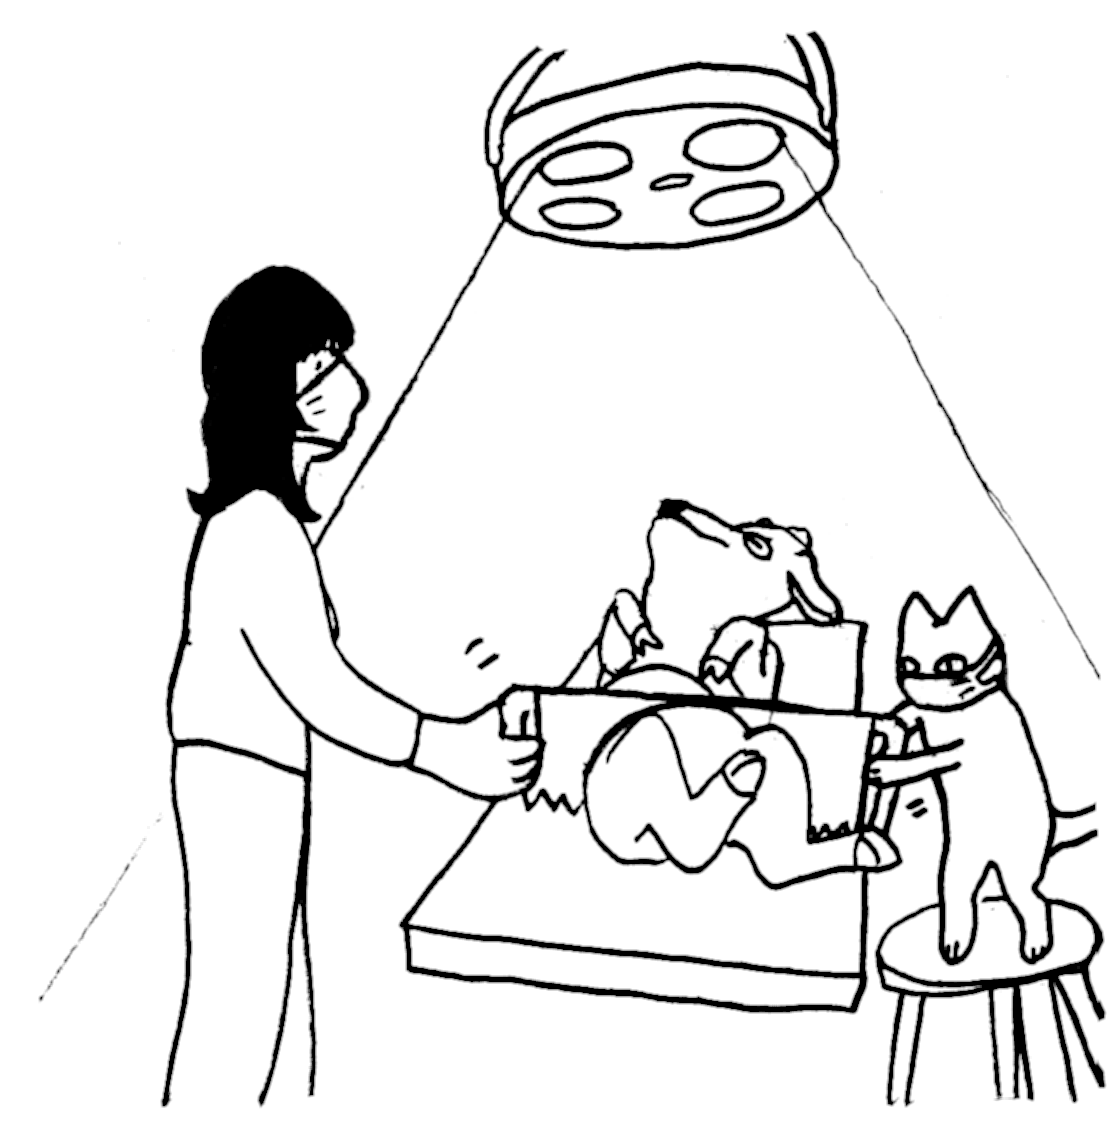
\includegraphics[width=0.5\textwidth]{pics/4.png}
&
  \begin{minipage}{0.45\textwidth}
    \vspace*{-35ex}
\begin{scriptsize}
 {%
 \leaf{\emph{I}}
 \branch{1}{NP}
 \leaf{\emph{saw}}
 \branch{1}{V:saw}
 \leaf{\emph{a}}
 \branch{1}{DET}
 \leaf{\makebox[1em]{\emph{kid} [goat]}}
 \branch{1}{N}
\branch{2}{NP}
 \leaf{\emph{with a cat}}
\branch{1}{PP[together]}
 \branch{3}{VP}
 \branch{2}{S}
 \qobitree}
\end{scriptsize}
\\[3ex]
 \small 
\iz{saw(I, kid: \textsc{present}) with(I, cat)}
\\[1ex] \iz{saw $\subset$ cut}
\\ \iz{kid $\sim$ young goat}
\\ \iz{with $\subset$ together}
\end{minipage}
\end{tabular}


\myslide{I saw a kid with a cat$_5$}
\hspace{-3em}\begin{tabular}{ll}
  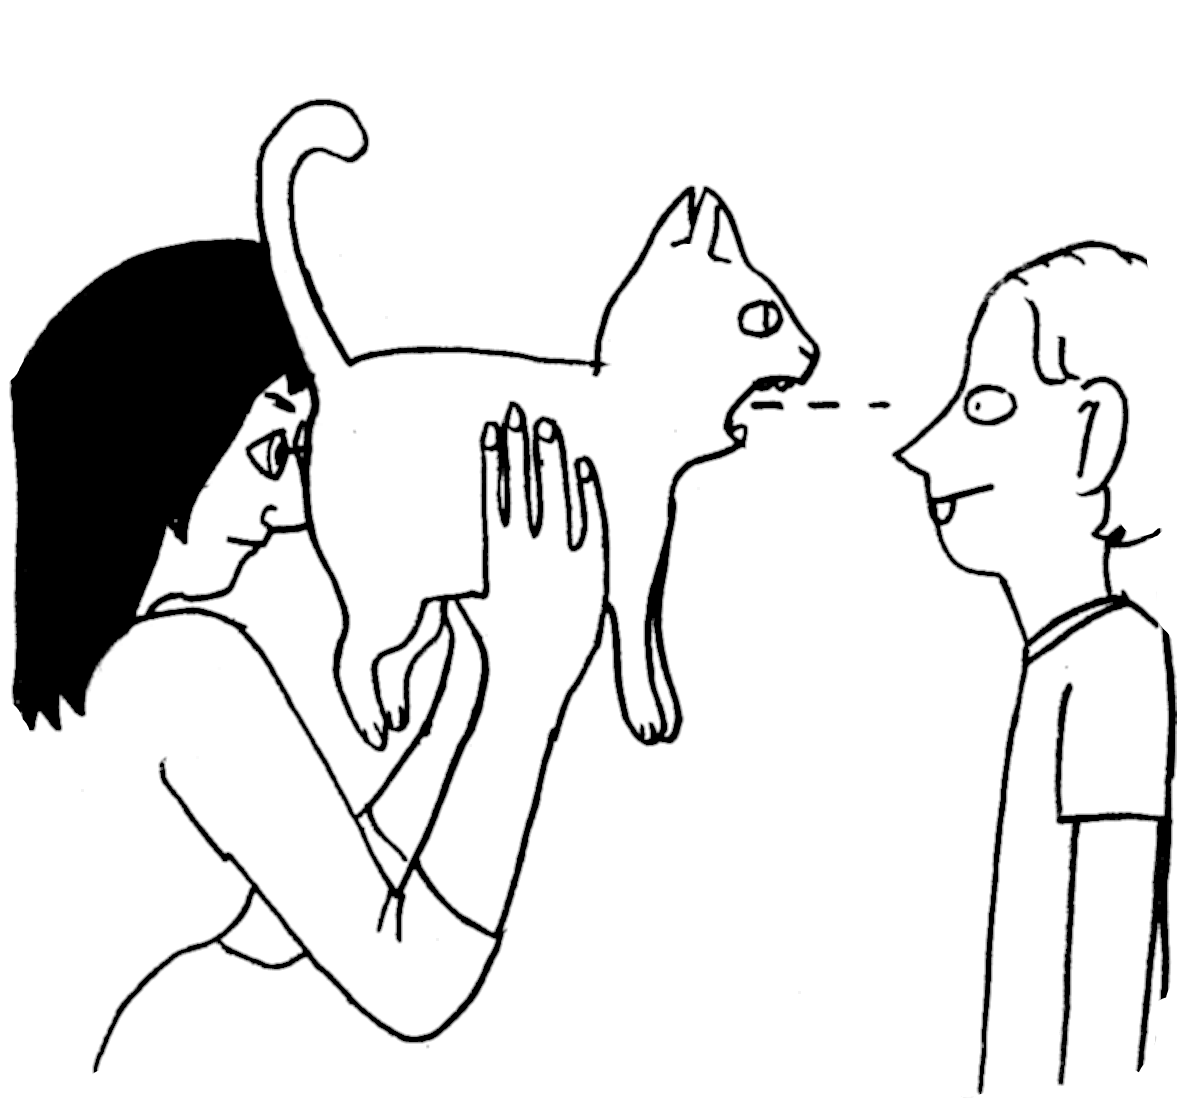
\includegraphics[width=0.5\textwidth]{pics/5.png}
&
  \begin{minipage}{0.45\textwidth}
    \vspace*{-35ex}
\begin{scriptsize}
 {%
 \leaf{\emph{I}}
 \branch{1}{NP}
 \leaf{\emph{saw}}
 \branch{1}{V:see}
 \leaf{\emph{a}}
 \branch{1}{DET}
 \leaf{\emph{kid}}
 \branch{1}{N}
\branch{2}{NP}
 \leaf{\emph{with a cat}}
\branch{1}{PP[instrument]}
 \branch{3}{VP}
 \branch{2}{S}
 \qobitree}
\end{scriptsize}
\\[3ex]
 \small 
 \iz{see(I, kid: \textsc{past}) with(I, cat) }
\\[1ex] \iz{see $\subset$ perceive}
\\ \iz{kid $\sim$ child}
\\ \iz{with $\subset$ instrumental}
 \end{minipage}
\end{tabular}


% \myslide{People are good at understanding}
% \MyLogo{We do this too}
% \begin{itemize}
% \item The words only hint at the meaning
% \item Many words can mean more than one thing (\blu{ambiguity})
% \item How can we \blu{model} and \blu{resolve} ambiguity?
% \item Look at the text and try to annotate the meaning
%   \begin{center}
%     Very hard work
%   \end{center}
% %   \begin{itemize}
% %   \item Deduce implicit models
% %     \begin{itemize}
% %     \item bag of words, $n$-gram chunks, \ldots
% %     \end{itemize}
% %   \item Define explicit models
% %     \begin{itemize}
% %     \item Grammars, lexicons and thesauri
% %     \end{itemize}
% %   \end{itemize}
% %\item Then build statistical language models (machine learning)
% \end{itemize}

\myslide{We can also use translations}
%\MyLogo{Work smarter}
%\addtocounter{exx}{-13}
\begin{exe}
  \ex \glll 我 看到了 一个 抱着 猫 的 孩子 \\
  wǒ   kàndàole    yīgè   bàozhe  māo  de    háizi. \\
  I saw one holding cat 's child \\
  \trans I did see a child holding a cat

  \ex \glll 我 抱着 猫 看到了 一个 孩子 \\
  wǒ  bàozhe māo kàndàole  yīgè     háizi \\
  I holding cat saw one  child \\
 \trans I holding a cat did see a child

  \ex \glll 我 鋸锯  一个 孩子 和 他/她 的 猫 \\
wǒ jù  yīgè    háizi  hé  tā/tā   de māo \\
%wo3 ju4  yi1ge4    háizi  he2  ta1ta1   de ma1o\\
 I      saw    one    child   and     he/she  's cat\\
 \trans I saw  a child and their cat 

  \ex \glll 我 和 一只 猫 鋸锯 一只 小 山羊 \\
wǒ hē  yīzhǐ  māo jù yīzhǐ xiǎo  shānyáng  \\
%wo3 he1  yi1zhi3  ma1o ju4 yi1zhi3 xia3o  sha1nya2ng    \\
I and one cat saw one small goat \\

\trans I and a child saw a young goat
  \ex \glll 我 用 一只 猫 看到了 一个 孩子 \\
wǒ yòng yīzhǐ  māo kàndàole  yīgè  háizi \\
I use one cat saw one child \\
\trans Using a cat, I did see a child
\end{exe}

\bigskip
\begin{center} \large
  Your turn: try to paraphrase --- translate into English
  \\ aim to be unambiguous, even if slightly disfluent\task
\end{center}

\myslide{Summary}
\MyLogo{Almost done}
\begin{itemize}
\item Syllabus; Administrivia
\item What is semantics?
\item Why should we be interested in semantics?
\item What is meaning?
\item Meaning as an open ended conceptual system
\item Semantic problems and solutions?
%\item Information Theory (new!)
\end{itemize}




\myslide{Administrivia}
\begin{description}\addtolength{\itemsep}{-5mm}
\item [Coordinator]  Francis \ul{Bond} 
{\small \url{<bond@ieee.org>} !\url{<fcbond@ntu.edu.sg>}}
% \item [Tutor]  James Sneed \ul{German}, Joanna \ul{Sio} Ut Seong 
% {\small \url{<jsgerman@ntu.edu.sg; neosome@gmail.com>}}
\item Details will all be  online:
  \begin{center}
    \url{https://bond-lab.github.io/Detecting-Meaning/}    
  \end{center}
\end{description}

\myslide{Assessment: On-line analysis}
\MyLogo{As this is only the second time there may be some glitches}
\begin{enumerate}
\item Disambiguation (20\%: individual work)
  \\ Identify and annotate word meaning for your own passage of one of the stories using wordnet as the sense inventory.
\item Comparison (20\%: group work)
  \\ Compare and contrast your annotations with other annotators; re-annotate based on your discussion and leave comments for at least five words.
\item Sentiment or Metaphor (20\%: individual work)
  \begin{itemize}
  \item  Identify and annotate sentiment for concepts from your own
  passage.
\item  Identify and annotate examples of metaphor from a new story
\end{itemize}

\end{enumerate}

\myslide{On-line Analysis}
\MyLogo{Read and enjoy!}
You will be assigned two short passages: one already annotated, and
one not.  During class discussions and for the projects you should try
to find examples from these.

Your homework this week is to read the following three stories, all
linked to from the main page:
\begin{itemize}\addtolength{\itemsep}{-2ex}
\item SPEC \textit{The Adventure of the Speckled Band} by
  Doyle, Arthur Conan (1892)
\item DANC \textit{The Adventure
  of the Dancing Men} by Doyle, Arthur Conan (1903) 
\item FINA \textit{The  Final Problem}
   by Doyle, Arthur Conan (1893) 
\end{itemize}

Next week I will reveal the endings (\emp{spoilers}) and you need to know the stories to follow the discussions.

\myslide{Assessment: Quizzes (40\%)}
\begin{itemize}
\item Quiz 1 (20\%)
  \begin{itemize}
  \item     Identifying characteristics of modern detective fiction
  \item     Identifying and analyzing key passages and characters from the assigned texts
  \item     Demonstrating an understanding of how narrative (and literary) devices function in Sherlock Holmes’ short stories
  \item     Considering how cultural and historical contexts shape and influence the stories
  \item     Understanding how popular culture takes, reshapes and extends 
  \end{itemize}
\newpage
\item   Quiz 2 (20\%)
  \begin{itemize}
  \item      Identifying and analyzing key scenes and characters from the assigned videos
  \item     Demonstrating an understanding of how narrative (and literary) devices function in Sherlock Holmes’ short stories
  \item     Demonstrating an understanding of how video differs from text in how stories are structured
  \item     Considering how cultural and historical contexts shape and influence the stories 
  \end{itemize}
\end{itemize}


\myslide{Extra Credit}

\begin{itemize}
\item If you submit a correction that gets accepted for one of the
  resources we use then it shows good mastery of the material
  \begin{itemize}
  \item you can get 1-5\% extra credit (depending on the size/difficulty)
\\ Mark $n \propto 10^{n-1}$ lines of code/documentation
  \item You can't go over 100\%
  \end{itemize}
\item A correction can involve
  \begin{itemize}
  \item fixing an error in transcription or annotation
    \begin{itemize}
    \item spelling error
    \item wrong sense
    \item error in the dictionary
    \end{itemize}
  \item making the documentation easy to read
  \item pointing out an error in a translation
%  \item  fixing a bug in code
%  \item extending the code with new capabilities
  \end{itemize}

\end{itemize}



\myslide{Student Responsibilities}

By remaining in this class, the student agrees to:
\begin{enumerate}
\item  Make a good-faith effort to learn and enjoy the material.
\item  Read assigned texts and participate in class discussions and activities.
\item Submit assignments on time.
\item Attend class at all times, barring special circumstances (see below).
\item Get help early: approach us when you first have trouble understanding a concept or homework problem rather than complaining about a lack of understanding afterward.
\item Treat other students with respect in all class-related activities, including on-line discussions.
\end{enumerate}
\myslide{Attendance}
\begin{enumerate}
\item You are expected to attend all classes.
\item Be on time - lateness is disruptive to your own and others' learning.
\item Valid reasons for missing class include the following:
\begin{enumerate}
\item A medical emergency (including mental health emergencies)
\item A family emergency (death, birth, natural disaster, etc).
\end{enumerate}
You must provide documentation to the student office.
\item There will be significant material covered in class that is not in your readings.  You cannot expect to do well without coming to class.
\item If you miss a class, it is your responsibility to get the notes, any handouts you missed, schedule changes, etc. from a classmate.
\end{enumerate}

\myslide{Remediation and Academic Integrity}
\begin{enumerate}
\item No late work will be accepted, except in the case of a documented excuse.
\item For planned, justified, absences on class days or days on which assignments are due, advance notice must be provided.
\item Cheating will not be tolerated. Violations, including plagiarism, will be seriously dealt with, and could result in \textbf{a failing grade for the entire course}.
\item Refer to the University Honour Code: 
\\ \url{http://academicintegrity.ntu.edu.sg/}
\item As always, use your common sense and conscience.
\end{enumerate}


\myslide{The winning strategy}

\begin{itemize}
\item Read the stories before class (and after again, if necessary)
\item Work together: make study groups
\item Tasks: Discuss as much as you want (but not project 1), annotate your own answers
\item Exams: No discussion
\item Ask questions \ldots\ early and often!
\end{itemize}


% \emp{Next Week}	Theories of meaning and the meaning of words

% \myslide{Acknowledgments and References}
% \MyLogo{If I have seen further, it is by standing on the shoulders of giants (Isaac Newton)}
% \begin{itemize}
% \item Course design and slides inherit from Nala Lee's HG202 course,
%   back in the depths of time (2009).
% \item Thanks to Na-Rae Han for 
%   inspiration for the student policies (from  \textit{LING 2050 Special Topics in Linguistics: Corpus linguistics}, U Penn; adapted).
%   \item Further Reading: 
%   \begin{itemize}
%   \item  Shannon, C.E. (1948), "A Mathematical Theory of Communication", Bell System Technical Journal, 27, pp. 379–423 \& 623–656, July \& October, 1948. \url{http://cm.bell-labs.com/cm/ms/what/shannonday/shannon1948.pdf}
%   \end{itemize}
% \end{itemize}



\end{document}

%%% Local Variables: 
%%% coding: utf-8
%%% mode: latex
%%% TeX-PDF-mode: t
%%% TeX-engine: xetex
%%% End: 

